\section{Graph Minors 1}

\subsection[Minors 1 - 1]{Prove that every 3-connected graph contains $K_4$ as a minor.}

Let $G = (V,E)$ be a 3-connected graph.
Using Menger's theorem the following claim holds:
\begin{claim}
    A graph $G$ is $k$-connected if and only if for every pair $u,v \in V(G)$ of non-adjacent vertices, there are $k$ internally disjoint ($u-v$)-paths in $G$.
\end{claim}
Let now $u,v \in V(G)$ be two non-adjacent vertices, and $P_1, P_2, P_3$ three internally disjoint $(u-v)$-paths.

Let $S$ be the shortest path between all pair of internal vertices in $P_1$, $P_2$, and $P_3$.
This is, have $S$ join the two closest internal vertices in the disjoint paths.

W.l.o.g. let $p \in V(P_2) \backslash \{u, v \}$ and $q \in V(P_3) \backslash \{ u, v\}$ be the end vertices of $S$.
If $V(S) \cap V(P_1) \neq \emptyset$, take $z \in V(S) \cap V(P_1)$ and taking the subpath $p-z$ or $z-q$ we reach a contradiction with the length of $S$.
Hence we have $V(S) \cap V(P_1) = \emptyset$.
Then $u,v,p,q$ (see supporting drawings) from a subdivision of $K_4$ (topological minor) and therefore $G$ has $K_4$ as a minor.
\begin{figure}[h!]
    \centering
    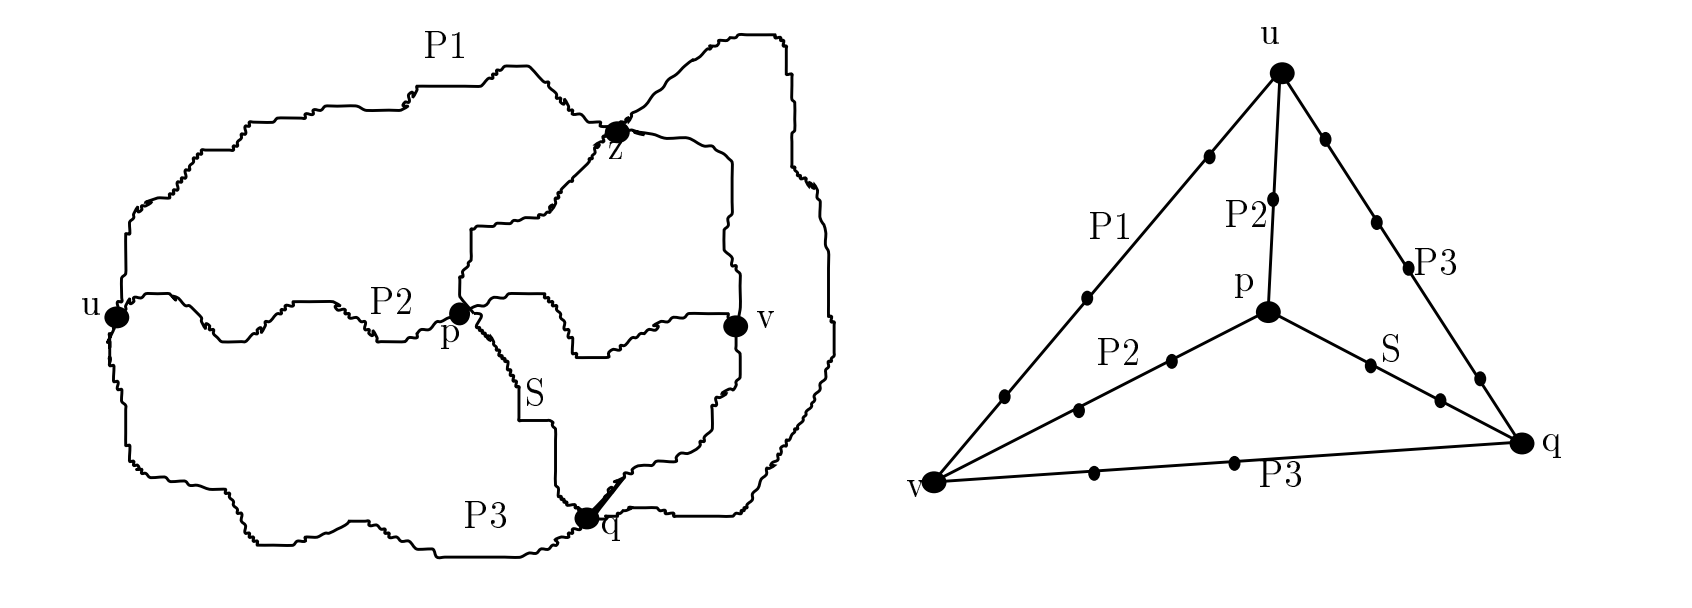
\includegraphics[width=\textwidth]{img/minors_1_1.png}
\end{figure}

\subsection[Minors 1 - 2]{Show that a graph is outerplanar if and only if it does not contain a subdivision of $K_4$ or $K_{2,3}$.}

Done - Problem 11 of Planar Graphs.

\subsection[Minors 1 - 3]{Show that a series-parallel graph with $n$ vertices has at most $2n -3$ edges. Show also that $\chi(G) \leq 3$.}

Let us start off with two definitions:
\begin{definition}[Edge Confluency]
    Two edges $e,f$ are \textbf{confluent} if there are no cycles $C, D$ in $G$ such that $C$ meets $e$ and $f$ in the same direction but $D$ meets them in the opposite.
\end{definition}

\begin{definition}[Series-Parallel Graph]
    A \textbf{series-parallel} graph can be defined either:
    \begin{itemize}
        \item Every pair of edges of $G$ are confluent.
        \item If and only if $G$ does not contain the complete graph $K_4$ as minor: $Forb(K_4)$.
    \end{itemize}
\end{definition}

We will prove the bound on the number of edges by induction on the number of vertices.
\begin{itemize}
    \item \textbf{Case n=3:} at most three edges, $3 \leq 2n - 3 = 1$
    \item \textbf{Inductive case:}
        Note that if $G$ does not contain $K_4$ as a minor and $n \geq 4$, there must exist $v \in V(G)$ such that $d(v) \leq 2$.
        Further, removing a vertex does not induce such a clique.
        Hence,
        $$E(G) \leq E(G \backslash v) + 2 \leq 2 V(G \backslash V) -3 + 2 = 2V(G) -3$$
\end{itemize}

The reason for the chromatic number is similar.
We proceed by induction: remove such vertex, color the graph, and then put it back in and assign one of the three colors.

\subsection[Minors 1 - 5]{Let $H$ be a graph. Show that there is a finite list $H_1, \dots, H_K$ of graphs such that a graph contains $H$ as a minor if and only if contains $H_i$ as a subdivision for some $i$.}

Let us firstly observe the following breakdown:
\begin{itemize}
    \item $\preceq$: can be decomposed in a series of edge contractions and edge deletion (taking subgraphs).
    \item $\preceq_{T}$: can be decomposed in a series of subdivisions and edge deletions.
\end{itemize}
Let us then observe that it suffices to prove that we can obtain H from G through a series of contractions because we could always arrange the intermediate graphs in such a way:
$$H \preceq H_N' \preceq \dots \preceq H_{k+1}' \preceq H_k' \preceq \dots \preceq H_1' \preceq G$$
such that $H_1', \dots, H_k'$ are deletions and $H_{k+1}', \dots, H_N'$ are contractions.
Because it is clear that if $G'$ is obtained from $G$ by deleting some edges, $G' \preceq_T G$.

\begin{definition}[Smoothing]
    Let $v \in V(G)$.
    \textbf{Smoothing:} $G$ at $v$ means replacing $v$ with two new vertices $v_1, v_2$ generating $G'$ such that:
    $$V(G') = V(G)\backslash \{v\} \cup \{v_1, v_2\} \quad E(G') = E(G)\backslash \{ vy \: : \: vy \in E(G) \} \cup \{ v_1y \vee v_2y \: : \: vy \in E(G) \}$$
    Note that smoothing is the inverse operation to contracting edges.
\end{definition}

\begin{definition}[Proper Smoothing]
    Given $v \in V(G)$, $d(v) \geq 4$, a \textbf{proper smoothing} of $G$ at $v$ is a smoothing such that $d(v_1), d(v_2) < d(V)$.
\end{definition}

\begin{definition}[Non-Proper Smoothing]
    Given $v \in V(G)$ if either:
    \begin{enumerate}
        \item We smooth $G$ at $v$ with $d(v) \leq 3$ or
        \item We smooth $G$ at $v$, $d(v) \geq 4$, and either $d(v_1) = d(v)$ or $d(v_2) = d(v)$
    \end{enumerate}
    we call this a \textbf{non-proper smoothing}.
\end{definition}

\begin{claim}
    The edge deletion induced by a non-proper smoothing is equivalent to a subdivision.
\end{claim}

As a consequence we can reduce our study to chains of proper smoothing.

Lastly, for the graph $H$ consider the set of all graphs $F_H$ such that after one contraction, we get $H$ as a minor.
$F_H$ is a finite set.
For each $H_i \in F_H$ consider the set $S_{H_i}$ consisting of all graphs obtained from $H_i$ by \textbf{properly smoothing} $H_i$ at any subset of appropriate vertices.
It remains to show that $F_H \cup (\cup_i S_{H_i}) \: \forall H_i \in F_H$ satisfies the statement.

\subsection[Minors 1 - 6]{Show that if $G$ is a $k$-sum of $G_1$ and $G_2$ then $\chi(G) \leq \max\{\chi{G_1}, \chi{G_2}\}$. Prove the Hadwiger conjecture for $t \geq 3$: if $\chi(G) > t$, then $G$ contains $K_{t+1}$ as a minor.}
